\documentclass[12pt]{article}
\usepackage[margin=0.5in]{geometry}
\usepackage{arev}
\usepackage{pgfplots}
\pgfplotsset{compat=1.17} % warning: the point plotting breaks at 1.10 and below

\begin{document}
\begin{figure}[h]
    \centering
    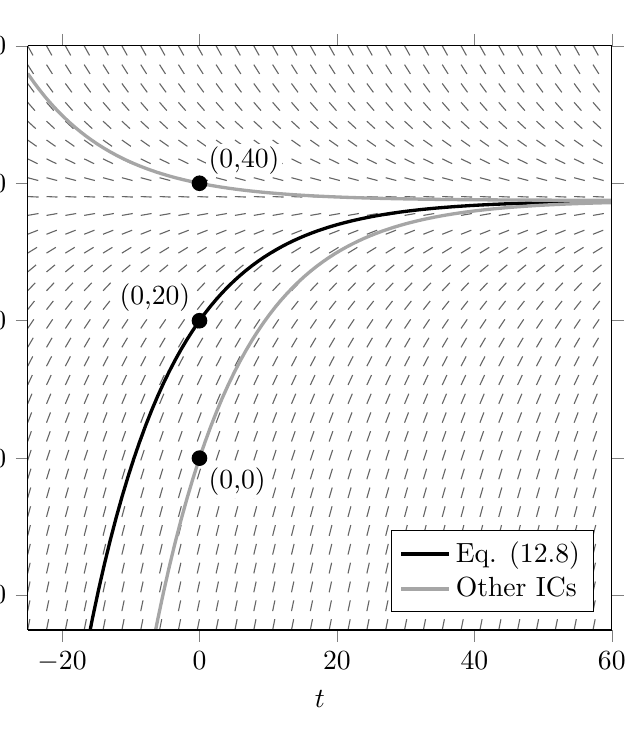
\begin{tikzpicture}[trim axis left, trim axis right] % options to centre correctly
        \def\dydx{3-0.08*y} % differential equation: dy/dx = f(x,y) => \def\dydx{f(x,y)}
        % this example has two solutions for a given `c`, i.e. parameter #1
        \newcommand\upperSolution[1]{(3+exp(-0.08*(x+#1)))/0.08} % for starting point above y=37.5
        \newcommand\lowerSolution[1]{(3-exp(-0.08*(x+#1)))/0.08} % for starting point below y=37.5

        % domain and tick settings - note domain is square, change in axis options if needed
        \def\domainMin{-25}
        \def\domainMax{60}
        \def\ticks{\domainMin+5,\domainMin+25,...,\domainMax} % define tick marks

        % #1: coordinates of node, #2: relative position of node label (can also be angle)
        \newcommand\labelledPoint[2]{\node[circle, fill, inner sep=2pt, label={[fill=white,distance=1pt,inner sep=1pt]#2:{(#1)}}] at (#1){}}

        \begin{axis}[view = {0}{90}, % set camera to point towards x-y plane
                     domain=\domainMin:\domainMax,
                     xmin=\domainMin, xmax=\domainMax,
                     ymin=\domainMin, ymax=\domainMax,
                     xlabel=$t$, ylabel=$w$,
                     xtick=\ticks, ytick=\ticks,
                     tick align=outside,
                     width=9cm, height=9cm,
                     legend pos=south east, legend cell align={left},
                     axis equal image]

            % plot unit length quivers with no head
            \addplot3[black!60, quiver={u=1/(sqrt((\dydx)^2+1)), v=(\dydx)/(sqrt((\dydx)^2+1)), scale arrows=1.6}, samples=32, forget plot] (x,y,0);

            % plot initial points and corresponding solution curves
            \addplot[very thick, black!100, samples=100] plot (x,\lowerSolution{12.5*(ln(5)-ln(7))});
            \labelledPoint{0,20}{above left};

            \addplot[very thick, black!35, samples=100] plot (x,\lowerSolution{-12.5*ln(3)});
            \labelledPoint{0,0}{below right};

            \addplot[very thick, black!35, samples=100] plot (x,\upperSolution{12.5*ln(5)});
            \labelledPoint{0,40}{above right};

            % add legend, ignoring quiver plot and the last solution curve
            \legend{Eq. (12.8), Other ICs}
        \end{axis}
    \end{tikzpicture}
    \caption{Slope field of $\frac{\mathrm{d}w}{\mathrm{d}t}=3-0.08w$ with solutions intersecting various initial conditions.}
\end{figure}
\end{document}
